\documentclass{book}
\usepackage{ctex}
\usepackage{xcolor}
\usepackage{hyperref}
\usepackage{graphics}

\title{\Large Git tutorial }

\author{LeeMoo}


\begin{document}

\maketitle
\tableofcontents
\subsection{}
The entire pro Git book, written by Scott Chacon and Ben Straub and published by Apress, is availble here. All conteent is licensed under the Creative Commons Attribution Non Commericial Share Alike 3.0 license. Print versions of the book are available on \href{www.amazon.com}{Amazon.com}.\\

\chapter{起步}
	\section{关于版本控制}
	\subsection{关于版本控制}
	\paragraph{}
	什么是版本控制?我为什么要关心它呢?版本控制是一种记录一个或若干个文件内容变化,以便将来查阅特定版本修订情况的系统。在配中所展示的例子中,我们仅对保存着软件源代码的广西文件作版本控制管理,但实际上,你可以对任何类型的文件进行版本控制。\\
	如果你是位图形或网页设计师,可能会需要保存某一幅图片或页面布局文件的所有修订版本(这或许是你非常渴望拥有的功能)。采用版本控制系统(VCS)是个明智的选择。有了它你就可以将某个文件回溯到之前的状态,你可以比较文件的变化细节,查出最后是谁修改了哪个地方,从而找出导致怪异问题的原因,又是谁在何时报告了某个功能缺陷等等.使用版本控制系统通常是意味着,就算你乱来一气把整个项目的文件改的改删的删,你也照样可以轻松恢复到原先的样子.但额外增加的工作量却微乎其微。\\
	\subsection{本地版本控制系统}
	\paragraph{}
许多人习惯用复制整个项目目录的方式来保存不同的版本,或许还会改名加上备份的时间以示区别.这么做唯一的好处就是简单.不过坏处也不少:有时候会混淆所在的工作目录,一旦弄错文件丢了数据就没法撤销恢复.\\
	为了解决这个问题,人们很久以前就开发了许多种本地版本控制系统,大多都是采用某种简单的数据库来记录文件的历次更新差异(如图1-1)。\\
	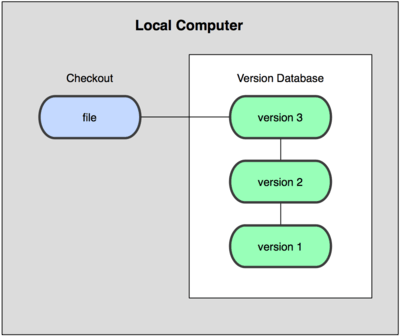
\includegraphics{1-1.png}\\
	\其中最流行的一种叫做RCS,现今许多计算机系统上都还看得到它的踪影.甚至在流行的Mac OSX 系统上安装了开发者工具包之后,也可以使用RCS命令.它的工作原理基本上就是保存并管理文件补丁(patch)。文件补丁是一种特定格式的广西文件,记录着对应文件修订前后的内容变化。所以,根据每次修订后的补丁,RCS可以通过不断打补丁,计算出各个版本的文件内容。\\
	\subsection{集中化的版本控制系统}
	\paragraph{}
	接下来人们又遇到一个问题,如何让在不同系统上的开发者协同工作?于是,集中化的版本控制系统(CVCS)应运而生.这类系统,诸如CVS,Subversion以及Perforce等,都有一个单一的集中管理的服务器,保存所有文件的修订版本,而协同工作的人们都通过客户端连到这台服务器,取出最新的文件或者提交更新.多年以来,这已成为版本控制系统的标准做法(见图1-2)\\
	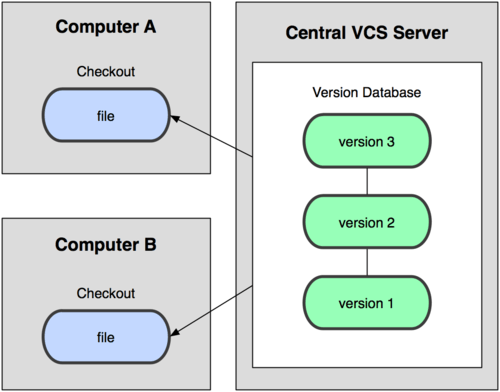
\includegraphics{1-2.png}\\
	这种做法带来了许多好处,特别是相较于老式的本地VCS来说。现在每个人都可以在一定程序上看到项目中的其他人正在做些什么.而管理员也可以轻松掌控每个开发者的权限,并且管理一个CVCS要远比在各个客户端维护本地数据库来得轻松容易。\\
	事分两面,有好有坏。这么做最显而易见的缺点是中央服务器的单点故障。如果宕机一小时,那么在这一小时内,谁都无法提交更新,也就无法协同工作.要是中央服务器的磁盘发生故障,碰巧没做备份,或者备份不够及时,就会有丢失数据的风险.最坏的情况是彻底丢失整个项目的所有历史更改记录,而被客户端偶然提取出来的保存在本地的某些快照数据就成了恢复数据的希望.但这样的话依然是个问题,你不能保证所有的数据都已经有人事先完整提取出来过.本地版本控制系统也存在类似问题,只要整个项目的历史记录被保存在单一位置,就有丢失所有历史更新记录的风险.\\
	\subsection{分布式版本控制系统}
	\paragraph{}
	于是分布式版本控制系统(DVCS)面世了。在这类系统中,像Git,Mercurial,Bazaar 以及Darcs等,客户端并不只提取最新版本的文件快照,而是把代码仓库完整地镜像下来.这么一来,任何一处协同工作用的服务器发生故障,事后都可以用任何一个镜像出来的本地仓库恢复。因为每一次的提取操作,实际上都是对代码仓库的完整备份(见图1-3)。\\
	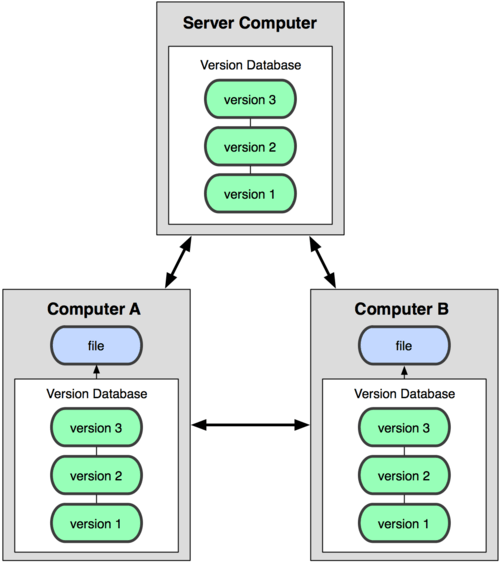
\includegraphics{1-3.png}\\
	更进一步,许多这类系统都可以指定和若干不同的远端代码仓库相互协作.你可以根据需要设定不同的协作流程,比如层次模型式的工作流,而这在以前集中式系统中是无法实现的.\\

	\section{Git简史}
	\subsection{Git简史}
	同生活中的许多伟大事件一样,Git诞生于一个极富纷争大举创新的年代。Linux内核开源项目有着为数众多的参与者.绝大多数的Linux内核维护工作都花在了提交补丁和保存归档的繁事务上(1991--2002年间)。到2002年,整个项目组开始雇用分布式控制系统BitKeeper来管理和维护代码。\\
	到了2005年,开发BitKeeper的商业公司同Linux内核开源社区的合作关系结束,他们收回了免费使用BitKeeper的权力。这就迫使Linux开源社区(特别是Linux的缔造者Linus Torvalds)不得不吸取教训,只有开发一套属于自己的版本控制系统才不至于重蹈覆辙。他们对新的系统制订了目标:\\
	\begin{itemize}
		\item 速度
		\item 简单的设计 
		\item 对非线性开发模式的强力支持(允许上千个并行开发的分支)
		\item 完全分布式
		\item 有能力高效管理类似Linux内核一样的超大规模项目(速度和数据量)
	\end{itemize}\\
	自诞生于2005年以来,Git日臻成熟完善,在高度易用的同时,仍然保留着初期设定的目标。它的速度飞快,极其适合管理大项目,它还有着令人难以置信的非线性分支管理系统(见第三章),可以就会各种复杂项目开发需求。\\


	\section{Git基础}
	\subsection{Git 基础}
	\paragraph{}
	那么,简单地说,Git空间是怎样的一个系统呢?请注意,接下来的内容非常重要,若是理解了Git的思想和基本工作原理,用起来就会知其所以然,游刃有余.在开始学习git的时候,请不要尝试把各种概念和其他版本控制系统相比拟,否则容易混淆每个操作的实际意义。Git在保存和处理各种信息的时候,虽然操作起来的命令形式非常相近,但它与其他版本控制系统的做法颇为不同.理解这些差异将有助于你准确地使用Git提供的各种工具。\\
	\subsection{直接记录快照,而非差异比较}
	\paragraph{}
	Git和其他版本控制的主要差别在于,Git只关心文件数据的整体是束发生变化,而大多数其他系统则只关心文件内容的具体差异。这类系统每次记录有哪些文件作了更新,以及都更新了哪些行的什么内容,请看图1-4。\\
	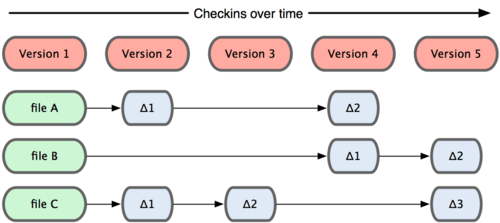
\includegraphics{1-4.png}\\
	Git并不保存这些前后变化的差异数据.实际上,Git更像是把变化的文件作快照后, 记录在一个微型的文件系统中.每次提交更新时,它会纵览一遍所有文件的指纹信息并对文件作一快照,然后保存一个指向这个快照的索引。为提高性能,若文件没有变化,Git不会再次保存,而只对上次保存的快照作一链接。Git的工作方式就像图1-5所示。\\
	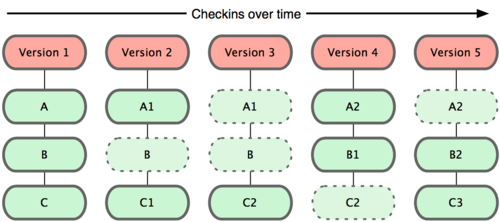
\includegraphics{1-5.png}\\
	这是Git同其他系统的重要区别.它完全颠覆了传统版本控制的套路,并对各个环节的实现方式作了新的设计。Git更像一个小弄的文件系统,但它同时还提供了许多以此为基础的超强的工具,而不只是一个简单的VCS。稍后在第三章讨论Git分支管理的时候,我们会再看看这样的设计空间会带来哪些好处。\\

	\subsection{近乎所有操作都是本地执行}
	在Git中的绝大多操作都只需要访问本地文件和资源,不用联网。但如果用CVCS的话,差不多所有操作都需要连接网络。因为Git在本地磁盘上就保存着所有当前项目的历史更新,所以处理起来速度飞快。\\
	举个例子,如果要浏览项目的历史更新摘要,Git不用跑到外面的用品上去取数据回来,而直接从本地数据库读取后展示给你看。所以任何时候你都可以马上翻阅,无需等待。如果想要看当前版本的文件和一个月之前的版本之间有何差异,Git会取出一个月前的快照和当前文件作一次差异运算,而不用请求远程来做这件事,或是把老版本的文件拉到本地来作比较。\\
	用CVCS的话,没有网络或者断开VPN你就无法做任何事情,但用Git的话,就算你在飞机或者火车上,
	\section{安装Git}
	\section{初次运行Git前的配置}
	\section{获取帮助}
	\section{小结}

\chapter{Git基础}
	\section{取得项目的Git仓库}
	\section{记录每次更新到仓库}
	\section{查看提交历史}
	\section{撤消操作}
	\section{远程仓库的使用}
	\section{打标签}
	\section{技巧和窍门}
	\section{小结}

\chapter{Git分支}

	\section{何谓分支}
	\section{分支的新建与合并}
	\section{分支的管理}
	\section{利用分支进行开发的工作流程}
	\section{远程分支}
	\section{分支的衍合}
	\section{小结}

\chapter{服务器上的Git}
	\section{协议}
	\section{在服务器上部署Git}
	\section{生成SSH公钥}
	\section{架设服务器}
	\section{公共访问}
	\section{GitWeb}
	\section{Gitosis}
	\section{Gitolite}
	\section{Git守护进程}
	\section{Git托管服务}
	\section{小结}

\chapter{分布式Git}
	\section{分布式工作流程}
	\section{为项目作贡献}
	\section{项目的管理}
	\section{小结}

\chapter{Git工具}
	\section{修订版本(Revision)选择}
	\section{交互式暂存}
	\section{储藏(Stashing)}
	\section{重写历史}
	\section{使用Git调试}
	\section{子模块}
	\section{子树合并}
	\section{总结}

\chapter{自定义Git}
	\section{配置Git}
	\section{Git属性}
	\section{Git挂钩}
	\section{Git强制策略实例}
	\section{总结}

\chapter{Git与其他系统}
	\section{Git与Subversion}
	\section{迁移到Git}
	\section{总结}
	
\chapter{git内部原理}
	\section{底层命令(Plumbing)和高层命令(Procelain)}
	\section{Git对象}
	\section{Git Refernces}
	\section{Packfiles}
	\section{The Refspec}
	\section{传输协议}
	\section{维护及数据恢复}
	\section{总结}



\end{document}
